\section{January 9, 2022}
\subsection{Introduction}
    Three main paradigms in modern Machine Learning\footnote{Additionally we also have reinforcement learning which is a very important paradigm and can be viewed as a hybrid between supervised and unsupervised learning}:
\begin{itemize}
    \item  Supervised learning 
    \item unsupervised learning 
    \item semi-supervised learning
\end{itemize}
Supervised learning is historically the oldest machine learning problem and it has a well-developed theory, methods and well-defined canonical formulation. Supervised learned basically amounts to learning some function $f$ via stochastic optimization.

$$
\text{Dataset} + \text{Algorithm} \to \text{Predictive Model}
$$





\subsection{Supervised learning}
Formally in supervised learning we are seeking $f:X \to Y$. 
$x \in X$ are instances, $y \in Y$ are labels. 
In classification problems $Y$ is a finite set, and in regression $ Y \subseteq \RR$. 
We obtain several $z_i = (x_i, y_i) \sim p$ on  $X \times Y$ labeled data which are generally referred to as samples or examples.
Our objective is to ``learn" $f$ and we accomplish by utilizing the \vocab{Empirical Risk Minimization} framework via using some loss function denoted by $V(f,z)$.

Examples of Loss Functions: 
\begin{itemize}
    \item Least squares loss $V(f,z) = (y - f(x))^2$
    \item Miss-classification (0-1) loss $V(f,z) = 0$ if sign is correct, otherwise $1$
    \item Hinge loss (or losgistic loss) $V(f,z) = log(1 + e^{-yf(x)})$
\end{itemize}

\subsection{Empirical Risk Minimization}
The ERM approach comes from empirical process theory (i.e, control theory).
Our objective is to seek $f \in \SF$ that minimizes \textbf{risk} (i.e., expected loss) :
$$
\SR (f) = \EE_{p} V(f,z)
$$
We use sample average as a stand-in estimator for the true risk, and minimize the \textbf{training error} in order to minimize the true risk $\SR(f)$:
$$
 \hat{\SR(f)} = \underset{f \in \SF}{\text{min}} \frac{1}{n} \sum_{i=1}^{n}V(f,z_i)
$$.

\subsection{Manifold learning}
\begin{itemize}
    \item learn manifold coordinates
    \item will be minimizing some quantity computed on random samples
\end{itemize} 
\begin{center}
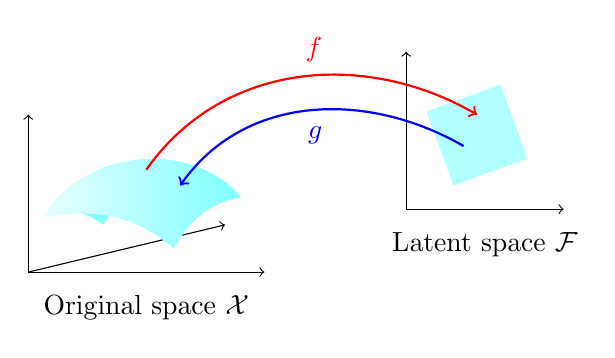
\begin{tikzpicture}
\definecolor{green}{rgb}{0.0, 1.0, 1.0}
\draw[->] (0, 0) -- ++(0, 2);
\draw[->] (0, 0) -- ++(2.5, 0.6);
\draw[->] (0, 0) -- ++(3, 0) node[midway, below, yshift=-0.5em]
    {Original space ${\cal X}$};

\draw[fill=green!50, draw=none, shift={(0.2, 0.7)},scale=0.5]
  (0, 0) to[out=20, in=140] (1.5, -0.2) to [out=60, in=160]
  (5, 0.5) to[out=130, in=60]
  cycle;

\shade[thin, left color=green!10, right color=green!50, draw=none,
  shift={(0.2, 0.7)},scale=0.5]
  (0, 0) to[out=10, in=140] (3.3, -0.8) to [out=60, in=190] (5, 0.5)
    to[out=130, in=60] cycle;

  \draw[->] (4.8, 0.8) -- ++(0, 2);
  \draw[->] (4.8, 0.8) -- ++(2, 0) node[midway, below, yshift=-0.5em]
      {Latent space ${\cal F}$};

  \draw[thin, fill=green!30, draw=none, shift={(5.4, 1.1)}, rotate=20]
    (0, 0) -- (1, 0) -- (1, 1) -- (0, 1) -- cycle;

  \draw[thick,->,red]
    (1.5, 1.3) to [out=55, in=150] node[midway, above, xshift=6pt, yshift=2pt]
    {$f$} (5.7, 2);

  \draw[thick,->,blue] (1.5, 1.3) ++(4.03, 0.3) to [out=150, in=55]
    node[midway, below, xshift=2pt, yshift=-2pt] {$g$} ++(-3.6, -0.5);

\end{tikzpicture}
\end{center}

\begin{center}
    
\end{center}

